\documentclass[border=5pt]{standalone}
\usepackage{fontspec}
\setmainfont{Times New Roman}
\setmonofont{Courier New}
\usepackage{amsmath,graphicx}
% Shared by the report and the standalone code figure generators.
\usepackage{xcolor,listings}

\definecolor{codeKeyword}{HTML}{174EA6}
\definecolor{codeBuiltin}{HTML}{6F3296}
\definecolor{codeIdentifier}{HTML}{243B53}
\definecolor{codeString}{HTML}{9C3328}
\definecolor{codeComment}{HTML}{396B45}
\definecolor{codeAddition}{HTML}{246B35}
\definecolor{codeDeletion}{HTML}{A12E2E}
\definecolor{codeDiffHeader}{HTML}{176B7D}

\lstdefinestyle{report-code}{
  basicstyle=\ttfamily,
  keywordstyle=\color{codeKeyword},
  keywordstyle=[2]\color{codeBuiltin},
  commentstyle=\color{codeComment},
  stringstyle=\color{codeString},
  identifierstyle=\color{codeIdentifier},
  columns=fullflexible,
  keepspaces=true,
  showspaces=false,
  showstringspaces=false,
  showtabs=false,
  upquote=true,
  tabsize=4,
  numbers=none,
  breaklines=false,
  aboveskip=0pt,
  belowskip=0pt,
  nolol=true
}

\lstdefinestyle{report-python}{
  style=report-code,
  language=[3]Python
}

\lstdefinestyle{report-bash}{
  style=report-code,
  language=bash,
  morekeywords={git}
}

\lstdefinelanguage{ReportDiff}{
  morekeywords={diff,index,git},
  moredelim=[l][\color{codeAddition}]{+},
  moredelim=[l][\color{codeDeletion}]{-},
  moredelim=[l][\color{codeDiffHeader}]{@@}
}
\lstdefinestyle{report-diff}{
  style=report-code,
  language=ReportDiff
}

\setlength{\fboxsep}{7pt}
\setlength{\fboxrule}{0.5pt}
\begin{document}
\begin{minipage}{510pt}
\fontsize{10}{12}\selectfont
\begin{minipage}[t]{246pt}
\vspace{0pt}\textbf{Python: addition creates an owned requirement}\par\smallskip
\begin{lstlisting}[style=report-python,basicstyle=\ttfamily\fontsize{8}{10.24}\selectfont]
protector = eps.add(Protection("protector"))
protector.undervoltage_threshold = 2.5
protector.overvoltage_threshold = 5.5
protector.current_limit = 1.0
protector.no_trip.voltages = "(3.3, 3.7)"
protector.no_trip.currents = "(0.0, 0.1)"
assert protector.no_trip.verify().verified is True
\end{lstlisting}
\end{minipage}\hfill\begin{minipage}[t]{252pt}
\vspace{0pt}\textbf{GUI: requirement owned by protector}\par\smallskip
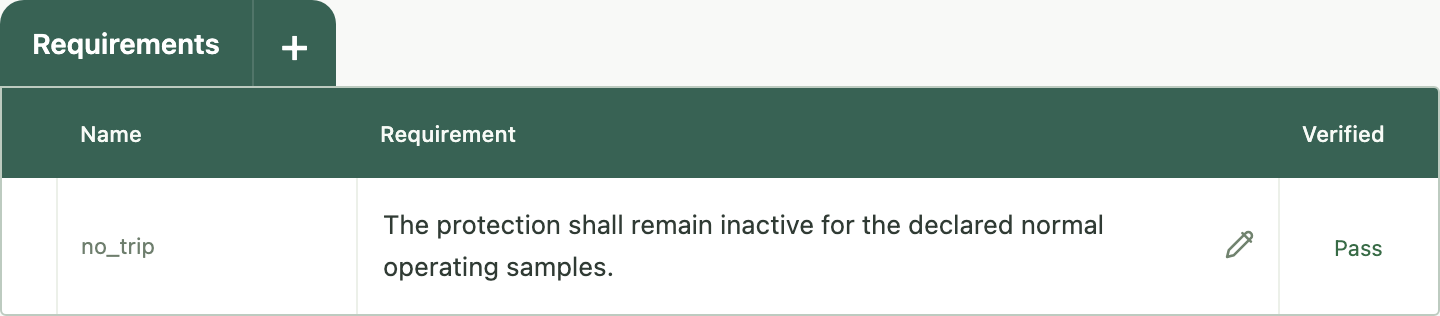
\includegraphics[width=252pt]{component-requirements.png}\end{minipage}\par\medskip\begin{minipage}[t]{506pt}
\vspace{0pt}\textbf{Source excerpt: automatic assignment hook}\par\smallskip
\begin{lstlisting}[style=report-python,basicstyle=\ttfamily\fontsize{8}{10.24}\selectfont]
class Protection(PowerCircuit):
    def create_requirements(self):
        # Threshold checks defined above (omitted).
        self.add_requirement(
            "no_trip",
            statement="The protection shall remain inactive for the declared normal operating samples.",
            # Rationale omitted.
            voltages=Property(unit="V"),
            currents=Property(unit="A"),
            conditions=tuple(conditions),
        )
\end{lstlisting}
\end{minipage}
\end{minipage}
\end{document}
